% The Free Flip. ATTRIB @ NeurIPS 2026 workshop submission (non-archival).
% Draft v3, 2026-08-17, on the neurips_2026 style. Every number's provenance is in
% NUMBERS.md; nothing here is quoted from memory.
% House style for this document: no em dashes and no prose colons.

\documentclass{article}

% ATTRIB is a NeurIPS workshop, so this uses the workshop track rather than the main
% conference track. `dblblindworkshop` keeps the submission anonymous, which matches the
% author block below and the fact that the authors of the replicated work may review this.
% If ATTRIB turns out to be single-blind, change this one word to `sglblindworkshop` and
% de-anonymise \author -- nothing else in the document depends on it.
\usepackage[dblblindworkshop]{neurips_2026}
\workshoptitle{Attributing Model Behavior at Scale (ATTRIB)}

\makeatletter
% Two corrections to the style's submission defaults, both because this is a WORKSHOP paper.
%
% 1. Under the anonymous option the style hardcodes a four-line placeholder block reading
%    "Anonymous Author(s) / Affiliation / Address / email" and ignores \author entirely
%    (neurips_2026.sty l.336). `@anonymous` is tested in exactly that one place, so clearing
%    it hands control back to \author with no other effect. Anonymity is then whatever
%    \author says, which below is the author line alone with no affiliation scaffolding.
% 2. The first-page footer defaults to the main-conference notice, "Submitted to ... NeurIPS
%    2026. Do not distribute.", which is not what an ATTRIB submission is. The style already
%    builds the right workshop line in `@trackname` but only emits it in camera-ready mode,
%    so we point the notice at it.
\@anonymousfalse
\renewcommand{\@noticestring}{\@trackname}
\makeatother

\usepackage[T1]{fontenc}
\usepackage[utf8]{inputenc}
\usepackage{booktabs}
\usepackage{amsmath,amssymb}
\usepackage{graphicx}
\usepackage{xcolor}
\usepackage{pgfplots}
\pgfplotsset{compat=1.18}
\usetikzlibrary{arrows.meta}
\definecolor{flipteal}{HTML}{2C6E8A}
\definecolor{failred}{HTML}{B03A2E}
\usepackage{microtype}
\usepackage[hidelinks]{hyperref}
% neurips_2026 loads natbib itself; only the style needs setting.
\bibliographystyle{plainnat}

\newcommand{\arm}[1]{\texttt{#1}}
\newcommand{\ci}[2]{{\small[#1,\,#2]}}

\title{The Free Flip. Reverse Capability in Obfuscation Fine-Tuning\\
Comes from Data Direction, Not a Contrastive Objective}

\author{Anonymous Author(s)}

\begin{document}
\maketitle

\begin{abstract}
Code obfuscation rewrites a program so that it still computes the same thing but is much
harder to read. A model can be trained to \emph{apply} such a rewrite, the forward
direction, or to \emph{undo} one, the reverse direction.
\citet{nikiema2025contrastive} report that fine-tuning on the forward direction destroys
the reverse direction, a failure they name \emph{cognitive specialization}, and propose
Contrastive Fine-Tuning as a remedy that recovers 39--52\% of reverse performance without
reverse training data. The auxiliary instances that objective requires are themselves new
data, so we test the two factors separately. In a $2\times2$ experiment on
Qwen2.5-Coder-1.5B the objective is worth $-0.2$ percentage points (95\% confidence
interval $[-0.7,+0.3]$) while reversing the data is worth $+30.9$ points
$[+29.3,+32.6]$. Reverse examples cost nothing to obtain, because every training pair read
backwards is one, and at 7B an arm that replaces half the forward pairs with their reverses
takes reverse success from $0.0\%$ to $32.8\%$ at identical training cost. Our
reimplementation of the published method reaches $0.1\%$, below the untouched model's
$12.9\%$. We differ from the original in language, corpus size and one transform, so we claim
non-reproduction on our corpus rather than in general. The recovered capability is narrower than reported, being at or below $2.3\%$ on
all three renaming transforms for every arm we trained, including reverse-only training.
The 6 to 7 point drop we measure on a general coding benchmark is also not caused by the
reverse data, since an arm trained on reverse data alone reaches the same reverse success
and shows no drop. The general pattern we would draw attention to is that fine-tuning on one
direction of a reversible transformation removes the other direction, and does so
selectively, leaving general coding ability intact at 7B while reverse success falls from
$12.9\%$ to $0.0\%$. The missing direction is then unusually cheap to restore, because its
training data is the data already in hand read backwards.
\end{abstract}

\section{Introduction}

\textbf{Directional training and the direction it removes.} Many useful code
transformations are reversible in principle. Obfuscating a program rewrites it so that it
behaves identically but is hard to read, by renaming \texttt{total\_price} to
\texttt{v\_a3f2} or by replacing a function's control flow with a dispatch loop. Each such
rewrite has a before and an after, so a model can be asked to work in either of two
directions (Figure~\ref{fig:attribution}). In the \textbf{forward} direction it is given
readable code and must produce the obfuscated version. In the \textbf{reverse} direction it
is given obfuscated code and must recover something readable and equivalent, which is the
direction practitioners actually want.

% The paper's central diagram. Hand-authored TikZ rather than an image so it sets in the
% document's own fonts and survives a style change. Both panels are deliberately identical
% except for the loss and the direction of the second arrow, because that is the whole point.
%
% Geometry note: the vertical gap between the two boxes has to be wide enough for the two
% arcs to read as a loop. A gap smaller than roughly the box height turns them into stubs.
\begin{figure}[t]
\centering
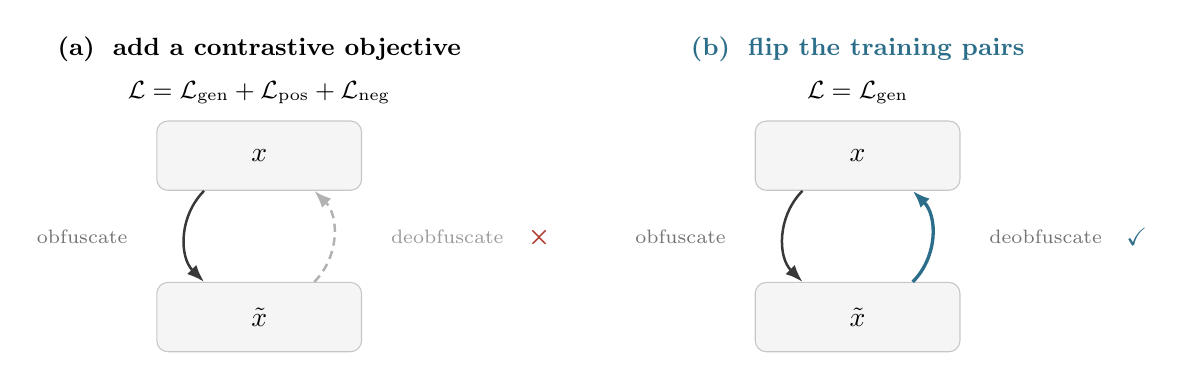
\begin{tikzpicture}[
  box/.style  ={draw=black!22, fill=black!4, rounded corners=4pt,
                minimum width=2.6cm, minimum height=0.88cm, font=\normalsize},
  hdr/.style  ={font=\small\bfseries},
  eqn/.style  ={font=\small},
  side/.style ={font=\scriptsize, text=black!55},
  vmark/.style ={font=\small\bfseries},
  fwd/.style  ={-{Latex[length=2.2mm]}, line width=0.9pt, black!78},
  dead/.style ={-{Latex[length=2.2mm]}, line width=0.9pt, black!30, densely dashed},
  live/.style ={-{Latex[length=2.2mm]}, line width=1.2pt, flipteal},
]

% ---------------- panel (a): the published intervention ----------------
\begin{scope}[shift={(0,0)}]
  \node[box] (ax)  at (0,2.05) {$x$};
  \node[box] (axo) at (0,0)    {$\tilde x$};
  \node[hdr] at (0,3.40) {(a)\; add a contrastive objective};
  \node[eqn] at (0,2.85)
    {$\mathcal{L}=\mathcal{L}_{\mathrm{gen}}+\mathcal{L}_{\mathrm{pos}}
                 +\mathcal{L}_{\mathrm{neg}}$};
  \draw[fwd]  ([xshift=-7mm]ax.south)  to[bend right=45] ([xshift=-7mm]axo.north);
  \draw[dead] ([xshift=7mm]axo.north) to[bend right=45] ([xshift=7mm]ax.south);
  \node[side, anchor=east] at (-1.55,1.02) {obfuscate};
  \node[side, anchor=west, text=black!40] (adl) at (1.55,1.02) {deobfuscate};
  \node[vmark, text=failred, anchor=west] at (adl.east) {\,\texttimes};
\end{scope}

% ---------------- panel (b): reading the same pairs backwards ----------------
\begin{scope}[shift={(7.6,0)}]
  \node[box] (bx)  at (0,2.05) {$x$};
  \node[box] (bxo) at (0,0)    {$\tilde x$};
  \node[hdr, text=flipteal] at (0,3.40) {(b)\; flip the training pairs};
  \node[eqn] at (0,2.85) {$\mathcal{L}=\mathcal{L}_{\mathrm{gen}}$};
  \draw[fwd]  ([xshift=-7mm]bx.south)  to[bend right=45] ([xshift=-7mm]bxo.north);
  \draw[live] ([xshift=7mm]bxo.north) to[bend right=45] ([xshift=7mm]bx.south);
  \node[side, anchor=east] at (-1.55,1.02) {obfuscate};
  \node[side, anchor=west] (bdl) at (1.55,1.02) {deobfuscate};
  \node[vmark, text=flipteal, anchor=west] at (bdl.east) {\,\checkmark};
\end{scope}

\end{tikzpicture}
\caption{The attribution this paper tests. Both panels fine-tune the same model on the same
obfuscation pairs. \textbf{(a)}~Contrastive Fine-Tuning augments the generation loss with two
equivalence-judgement terms and is credited with restoring the reverse direction. In our
experiments it does not. Reverse success stays at zero and falls below the untouched model.
\textbf{(b)}~Keeping the plain generation loss and reading half of the same pairs backwards
restores the reverse direction at identical training cost. The recovery comes from the
direction of the data, not from the objective.}
\label{fig:attribution}
\end{figure}


The phenomenon this paper is about is that fine-tuning on one of those directions removes
the other. At 7B, forward-only fine-tuning takes reverse success from $12.9\%$ to $0.0\%$.
The loss is also selective rather than a general degradation, which is what distinguishes it
from ordinary catastrophic forgetting. The same model keeps its general coding ability
completely intact, scoring $.817$ on HumanEval+ against $.805$ for the untouched model, so
what fine-tuning removed was specifically the inverse of the mapping it was taught. A
practitioner who fine-tunes a model to apply a transformation should expect to lose the
ability to undo it, and to lose it without any warning sign in general benchmarks.

\textbf{The reported remedy, and why it is an attribution problem.}
\citet{nikiema2025contrastive} document this failure, name it \emph{cognitive
specialization}, and propose \textbf{Contrastive Fine-Tuning} (CFT) as a remedy. CFT adds two
equivalence-judgement terms to the generation loss (Figure~\ref{fig:attribution}a), training
the model to say whether two programs are semantically equivalent alongside learning to
obfuscate. They report that this recovers 39--52\% reverse success \emph{without any reverse
training data}, which is what makes the result striking, because it suggests the capability is
unlocked by how the model is trained rather than by what it is shown.

That conclusion depends on an attribution that was not tested. CFT changes two things at
once, adding an objective and adding the equivalence-judgement instances that objective
requires, which are data the forward-only baseline never sees. A much cheaper candidate is
available too. Every training example pairs a readable program with an obfuscated one, so
reading a pair backwards is already a reverse example, obtained at no cost. If that alone
restores the reverse direction, then the failure describes the data a recipe was given
rather than the objective it was trained under. The original paper's evaluation section does
define a Bidirectional Fine-Tuning condition, forward generation plus reverse
deobfuscation, but reports no result for it, so we run that comparison here.

\textbf{What we find.} The data direction accounts for essentially the entire effect and the
objective for none of it (Figure~\ref{fig:attribution}b). A model trained on half forward and
half reversed pairs, at identical cost to forward-only training, goes from $0.0\%$ to $32.8\%$
reverse success, while our reimplementation of CFT reaches $0.1\%$. Two qualifications matter.
The recovered capability is confined to rewrites that can in principle be undone, and training
on both directions carries a general-capability cost that training on either one alone does
not, so the cheapest correct fix depends on whether both directions are needed at deployment.

\section{Setup}
\label{sec:setup}

\textbf{Programs and rewrites.} We use Python functions that come with executable test
inputs, drawn from APPS \citep{hendrycks2021apps}, CRUXEval \citep{gu2024cruxeval} and
HumanEval \citep{chen2021codex}. Each function is rewritten under five obfuscating transforms. Three rewrite identifiers, by
renaming them to misleading names (\arm{L1b}), to random strings such as \texttt{v\_a3f2}
(\arm{L1r}), or to single letters with type annotations stripped (\arm{L2}). Two rewrite
structure, by flattening control flow into a dispatch loop (\arm{S1}) or inserting
always-true tests and unreachable code (\arm{S2}). That split matters later, because only the
structural rewrites can be undone. Full definitions are in Appendix~\ref{app:conditions}.
Every rewrite is applied to the original function on its own, never stacked, and is kept only
if the rewritten program still produces the original outputs.

\textbf{How we score a trial.} For one trial let $x$ be the original readable program,
$\tilde x$ its obfuscated form, and $\hat y$ the model's output. Four quantities build the
criteria. $\mathrm{parses}(\hat y)$ is 1 when the output is non-empty and parses in the target
language. $S(a,b)\in[0,1]$ is CodeBLEU similarity between two programs
\citep{ren2020codebleu}. $R(a)\in[0,1]$ is readability, a weighted sum of identifier
meaningfulness (0.55) with identifier length, line length and nesting depth (0.15 each), and it
returns 0 for a non-parsing output, since the readability of a non-program is undefined and 0
is the only resolution that cannot manufacture a success. $E(\hat y)$ is 1 when the output
executes and reproduces $x$'s outputs on every test input that ships with the program.
Appendix~\ref{app:metrics} restates these as a table.

In the forward direction the model must emit an obfuscated program, and we score it by
whether that program still computes the original outputs, so forward success is $E(\hat y)$.

For the reverse direction we report two criteria, because the published one turns out to be
permissive. The \textbf{published criterion} is the test used by
\citet{nikiema2025contrastive}, which asks that the output be textually dissimilar to the
obfuscated input and about as readable as the original,
\begin{equation}
\mathrm{Pub}(\hat y) \;=\; \mathrm{parses}(\hat y) \;\wedge\;
\big[\,S(\hat y,\tilde x) < 0.4\,\big] \;\wedge\;
\big[\,R(\hat y) \ge R(x) - 0.1\,\big],
\label{eq:pub}
\end{equation}
where the thresholds are that paper's values and the $\mathrm{parses}$ conjunct is ours. The
guard is not optional, because without it the first inequality is satisfied by any reply that
merely differs from the input, and a run of fixed placeholder strings scored 17--25\% ``reverse
success'' before we added it. It can only lower a reported number, never inflate one.

\textbf{Strict success}, which we use for every headline number, additionally requires that
the recovered program run correctly,
\begin{equation}
\mathrm{Strict}(\hat y) \;=\; \mathrm{Pub}(\hat y) \;\wedge\; E(\hat y).
\label{eq:strict}
\end{equation}
We report it because a deobfuscation that does not run has not recovered anything. We also
track \textbf{echoing}, $\mathrm{Echo}(\hat y)=\mathbf{1}[\hat y = \tilde x]$, which is how
often the model simply returns its input, separately rather than letting such replies count
towards accuracy.

One substitution matters for Eq.~\eqref{eq:pub}. The original study measures readability with
the model of \citet{scalabrino2018comprehension}, which we do not have, so $R$ is the proxy in
Table~\ref{tab:metrics}. We checked what that costs by recomputing every result while varying
the readability treatment, including dropping the term entirely, and strict success moves by
at most $1.3$ pp on any trained arm against an effect of 33 points
(Appendix~\ref{app:fidelity}). Execution and the similarity bound do essentially all the
deciding.

\textbf{What we compare.} Every model in this paper is the same base model with a small
set of adapter weights trained on top, using LoRA \citep{hu2022lora}, and every one uses an
identical recipe (rank 32, three epochs, learning rate $10^{-4}$, batch 64, seed 17). The
only thing that differs between them is the mixture of training examples, so no difference
between them can come from hyperparameters. We call each mixture an \textbf{arm}, and
Table~\ref{tab:arms} lists them.

\begin{table}[t]
\centering\small
\caption{The training mixtures compared in this paper. Only the mixture differs; the model,
recipe and budget are otherwise identical. \arm{mix50} \emph{replaces} forward examples
rather than adding to them, which is what makes it cost the same as \arm{sft}.}
\label{tab:arms}
\begin{tabular}{llp{6.6cm}}
\toprule
arm & training examples & why it is in the experiment \\
\midrule
\arm{base} & none & the untouched control the original study omits \\
\arm{sft} & forward only & the original study's forward-only baseline \\
\arm{cft} & forward $+$ equivalence judgements & our reimplementation of the published method \\
\arm{flip} & forward $+$ the same pairs reversed & the declared but unreported baseline \\
\arm{mix50} & half forward, half reversed & the decisive arm, cost-matched to \arm{sft} with \emph{less} supervision \\
\arm{rev} & reverse only & how well reverse can be done at all \\
\arm{fwd2x} & forward only, twice the epochs & rules out ``it simply trained longer'' \\
\arm{cftflip} & judgements $+$ both directions & the fourth cell of the $2\times2$ \\
\bottomrule
\end{tabular}
\end{table}

\textbf{Evaluation and uncertainty.} We decode greedily on 300 held-out programs, using
only programs that every transform succeeded on so that no two cells are scored on
different populations. All intervals are 95\% confidence intervals from a bootstrap that
resamples \emph{programs} rather than individual test cases, because several test cases
share a program and are therefore correlated. We write \textbf{pp} for percentage points.
Greedy decoding is not bitwise repeatable here, since batching changes which token wins a
near-tie, so two passes over the same programs differ on 6 to 8\% of generations and move a
headline rate by about $0.2$ pp (Appendix~\ref{app:fidelity}). Every table comes from a single
pass, we compare arms only within a pass, and we never quote a cross-pass difference below
$0.5$ pp.

\section{The objective contributes nothing; the data direction contributes everything}
\label{sec:factorial}

Table~\ref{tab:factorial} varies the two factors CFT bundles together. One factor is
whether the equivalence-judgement objective is present. The other is whether the training
data contains the reversed pairs. All four cells use the same 300 programs and the same
18\,000 graded attempts.

\begin{table}[t]
\centering\small
\caption{The $2\times2$ experiment. Qwen2.5-Coder-1.5B \citep{hui2024qwen25coder}, strict
reverse success in per cent, 300 programs and 18\,000 graded attempts, all cells scored on
the same programs. The right-hand panel decomposes the four cells into the effect of each
factor.}
\label{tab:factorial}
\begin{tabular}{lcc}
\toprule
& forward only & $+$ reversed pairs \\
\midrule
no judgement objective & \arm{sft} \;\;0.3 & \arm{flip} \;\;\textbf{31.4} \\
with judgement objective & \arm{cft} \;\;0.3 & \arm{cftflip} \;\;\textbf{31.1} \\
\bottomrule
\end{tabular}
\hspace{1.5em}
\begin{tabular}{lcc}
\toprule
effect of & estimate (pp) & 95\% CI \\
\midrule
\textbf{reversing the data} & $\mathbf{+30.9}$ & $[+29.3,+32.6]$ \\
\textbf{the objective} & $\mathbf{-0.2}$ & $[-0.7,+0.3]$ \\
the two interacting & $-0.3$ & $[-1.3,+0.7]$ \\
\bottomrule
\end{tabular}
\end{table}

The objective's contribution is not merely too small to detect. It is bounded under one
percentage point in either direction, and that holds whether or not reversed data is
present, with an interaction term that also spans zero. Adding the judgement objective to
forward-only training moves reverse success by $-0.1$ pp $[-0.5,+0.3]$, and adding it on
top of reversed data moves it by $-0.3$ pp $[-1.2,+0.5]$. Reversing the data, by contrast,
moves it by roughly 31 points. Whatever recovers the reverse direction, it is not the
objective.

Training longer does not explain it either. \arm{fwd2x} trains forward-only for twice as
many optimizer steps and reaches $0.6\%$, which is $+0.3$ pp over \arm{sft} with an
interval of $[-0.2,+0.8]$.

\textbf{How much reversed data is needed, and it is much less than half.}
Appendix~\ref{app:dose} replaces forward examples with reversed ones in increasing amounts.
Replacing only 5\% of them already recovers $26.1\%$, against $0.3\%$ for forward-only,
which is 85\% of what a 50\% share achieves. The remaining climb is real but small, worth
$+4.5$ pp $[+3.2,+5.8]$, and it has flattened by the time a quarter of the data is
reversed. So the intervention is not a matter of data volume. A small amount of exposure to
the reverse direction captures most of the effect.


\section{The effect is free, at 7B, on every axis of training cost}
\label{sec:budget}

The obvious objection to Table~\ref{tab:factorial} is that \arm{flip} sees twice as many
examples as \arm{sft}. \arm{mix50} answers it by \emph{replacing} half the forward examples
with reversed ones instead of adding them, so it trains on the same number of examples
(7\,383) for the same number of optimizer steps (346). Two quantities are worth separating
here. \textbf{Sequence tokens} are all the tokens the model reads, which is what determines
compute. \textbf{Supervised tokens} are the subset the training loss is actually computed
on, which is what determines how much the model is taught. \arm{mix50} uses $1.05\times$
the sequence tokens of \arm{sft} and only $0.71\times$ the supervised tokens, so it is
taught \emph{less}, not more. Table~\ref{tab:main7b} reports both directions at 7B.

\begin{table}[t]
\centering\small
\caption{Qwen2.5-Coder-7B, 300 programs, 21\,000 graded attempts. \emph{Forward} is scored
by execution. \emph{Reverse (strict)} requires the published criterion and that the output
run correctly. \emph{Echo} is how often the model returns its input unchanged.}
\label{tab:main7b}
\begin{tabular}{lcccc}
\toprule
arm & forward & \textbf{reverse (strict)} & reverse (published crit.) & echo \\
\midrule
\arm{base} \emph{(untouched)}      & .929 & \textbf{.129} & .233 & .073 \\
\arm{sft} \emph{(forward only)}    & .971 & \textbf{.000} & .004 & .182 \\
\arm{fwd2x} \emph{(2$\times$ epochs)} & .969 & \textbf{.001} & .019 & .071 \\
\arm{cft} \emph{(published method)} & .975 & \textbf{.001} & .002 & \textbf{.293} \\
\arm{rev} \emph{(reverse only)}    & .927 & \textbf{.329} & .351 & .000 \\
\arm{flip}                         & .971 & \textbf{.335} & .353 & .000 \\
\arm{mix50} \emph{(same cost as \arm{sft})} & .961 & \textbf{.328} & .356 & .000 \\
\bottomrule
\end{tabular}
\end{table}

\arm{mix50} reaches $+32.8$ pp over \arm{sft} $[+31.3,+34.4]$ while costing no more on any axis
a practitioner pays for, and \arm{flip}, which does spend $2.09\times$ the sequence tokens,
buys only $+0.7$ pp more $[-0.3,+1.8]$, an interval spanning zero. The extra compute is not
what produces the capability. The exposure is. The published method fares worst here, spending
$2.65\times$ the compute of forward-only training to add 2\% more supervised signal, because
each equivalence judgement puts two whole programs in the prompt and supervises one word.

\textbf{The replication fails in the direction that matters.} Our \arm{cft} arm reaches
$0.1\%$ strict reverse success at 7B, against a reported 39--52\%. The gap is not merely a shortfall, since \arm{cft}
lands $12.8$ pp \emph{below the untouched model} $[-14.8,-10.9]$, which itself scores $12.9\%$,
and forward-only training lands equally far below. Both recipes \emph{remove} a capability the
base model already had, and the contrastive one does not restore it. We report this at 7B
because that is the size at which the original study's open-source results sit. Our corpus is
Python and smaller than theirs, so we claim the method does not reproduce here and that the
mechanism it was credited with is available for free.

\textbf{Where the fix does not work, and this is the main limit on ``free''.} The headline
$33\%$ averages five transforms that behave nothing alike, and the average conceals a hard
ceiling. On the two structural transforms the bidirectional arms reach about $80\%$. On the
three renaming transforms \emph{every} arm we trained sits at or below $2.3\%$, and that
includes \arm{rev}, which sees nothing but deobfuscation examples for the whole of training
(Appendix~\ref{app:bycond}). The reason is not a shortage of data or capacity but the task
itself. Once \texttt{total\_price} has been rewritten to \texttt{v\_a3f2}, the original name
is not present anywhere in the input, so no quantity of reverse supervision can recover it,
so a practitioner should not expect reverse training to help on transforms that destroy
information rather than rearrange it. The flip is free on budget, and it works only where the
transformation has an inverse left to learn.

A second correction concerns the measurement rather than the method. The published criterion
certifies very little, since outputs that pass it recover almost exactly as many original
identifiers as the model's outputs do in general (Appendix~\ref{app:e8}).

\section{What bidirectional training costs, and why that cost is also misattributed}
\label{sec:cost}

Calling the flip free is a claim about training budget, and we scope it that way. On
forward accuracy it is genuinely free, since \arm{flip} matches \arm{sft} on every transform
(Appendix~\ref{app:fwd}). On general coding ability it is not. We measure that with
HumanEval+ \citep{liu2023evalplus}, a benchmark of 164 standalone programming problems
scored by running the model's solution against tests, where \textbf{pass@1} is the fraction
solved on the model's first attempt.

\begin{table}[t]
\centering\small
\caption{HumanEval+ pass@1 (164 problems, no scorer errors in any cell), grouped by whether
the training mixture contains one direction of the rewrite or both. At 7B it is the
grouping, not the amount of reverse data, that predicts the cost.}
\label{tab:humaneval}
\begin{tabular}{lcc}
\toprule
arm & 1.5B & 7B \\
\midrule
\arm{base} \emph{(untouched)} & \textbf{.646} & \textbf{.805} \\
\midrule
\multicolumn{3}{l}{\emph{trained on ONE direction}} \\
\quad\arm{sft} \emph{(forward only)} & .329 & .817 \\
\quad\arm{fwd2x} \emph{(forward, 2$\times$ epochs)} & n/a & .805 \\
\quad\arm{cft} \emph{(forward $+$ judgements)} & .366 & .799 \\
\quad\arm{rev} \emph{(reverse only)} & .585 & \textbf{.799} \\
\midrule
\multicolumn{3}{l}{\emph{trained on BOTH directions}} \\
\quad\arm{flip} & .512 & \textbf{.744} \\
\quad\arm{mix50} & .469 & \textbf{.732} \\
\bottomrule
\end{tabular}
\end{table}

At 7B every arm trained on a \emph{single} direction lands within $1.2$ points of the
untouched model, including \arm{rev}, which is trained on reverse data exclusively. The two
arms carrying both directions lose 6 to 7 points. The comparison that isolates this is
\arm{rev} against \arm{mix50}. They use the same number of examples and optimizer steps,
\arm{rev} is taught \emph{less} ($0.43\times$ the supervised tokens against $0.71\times$),
and they reach the same reverse success ($32.9\%$ against $32.8\%$), yet \arm{mix50} gives
up $6.7$ points of pass@1 and \arm{rev} gives up none. Data volume, compute and reverse
exposure are all held level, so what is left is whether the model must learn a rewrite and
its inverse at the same time. This narrows the cost claim rather than removing it.
Bidirectional training costs 6 to 7 points; reverse data on its own does not.

Two cautions. The scales disagree, and at 1.5B the grouping fails, because forward-only
training is there the most damaging arm, which reads as ordinary overfitting to a narrow task.
And 104 of the 164 HumanEval+ problems have their reference solutions in our training corpus,
since HumanEval is one of its three sources, so every trained arm saw them while the untouched
model did not. Comparisons \emph{among} trained arms, which is what the grouping rests on, are
unaffected, but the $6$ to $7$ point figures against the untouched model are not clean.

\section{Related work}

\textbf{Directionality and the reversal curse.} The nearest literature to our phenomenon is
the reversal curse. \citet{berglund2024reversal} show that a model trained on ``A is B'' does
not thereby learn ``B is A'', and \citet{golovneva2024reverse} cure much of that failure with
reverse training, in which strings are additionally presented reversed, evaluated in both
data-matched and compute-matched settings. Our budget-matched arm is the same manoeuvre, and
their result is a reason to expect ours.

What we report is a different failure with the same symptom. The reversal curse is a failure to
\emph{generalize} to a direction never trained, so the capability was never present. Here the
untouched model can already work in reverse, scoring $12.9\%$ at 7B, and forward-only
fine-tuning \emph{removes} it, taking it to $0.0\%$. Destroying an ability the model had is not
the same event as failing to acquire one, and it is caused by the fine-tuning a practitioner
chooses to run. The loss is also selective, leaving general coding ability untouched, whereas
the reversal curse describes a limit on what a training distribution can teach rather than
damage to an existing skill. The inverse here is semantic too, undoing a program
transformation rather than reordering tokens or entities.

\textbf{Deobfuscation.} \citet{nikiema2025contrastive} is the study replicated here. A larger
literature trains models to recover source from a transformed form, whether obfuscated,
compiled or decompiled \citep{roziere2021dobf,tan2024llm4decompile,hu2026bindeobf}, and our
setting differs in where the reverse supervision comes from, since we re-read pairs that
already exist. \citet{guzman2026poisoned} find that misleading identifiers survive
deobfuscation almost always, agreeing with our renaming ceiling. All arms are LoRA adapters
\citep{hu2022lora}.

\section{Limitations and conclusion}
\label{sec:limits}

Our study is Python and JavaScript rather than Java, two sizes of one model family with the 7B
arms at a single seed, and five transforms rather than the original's three, and the
general-capability benchmark overlaps our training corpus. Appendix~\ref{app:limits} has the
full list.

Fine-tuning a model on one direction of a reversible code transformation removes the other
direction, and removes it selectively, leaving general coding ability untouched at 7B while
reverse success falls to zero. That is the finding a practitioner should carry away, because
a directional blind spot of this kind will not show up in a general benchmark. It is also
cheap to prevent, since the training data for the missing direction is the data already in
hand read backwards, and an arm that replaces half its forward examples with reversed ones
recovers the direction at no additional training cost.

The remedy proposed for this failure in prior work is credited to the wrong factor, since the
recovery comes from the reverse data it supplies rather than from its objective, and the cost is
misattributed the same way. A factor credited with an effect should be tested against the
ablation its own training instances supply.

\bibliography{refs}

% Order required by the NeurIPS template: references, then supplemental material, then the
% checklist. Neither the appendix nor the checklist counts toward the page limit.
\appendix
\section*{Appendix}

\section{Reimplementation fidelity, deviations, and the determinism floor}
\label{app:fidelity}

\paragraph{The original objective is instance-level.} (i) Its three terms are described
only as instance pools with counts (``30\,000 instances, 10\,000 each for positive
classification, negative classification, and obfuscation task generation''); the words
InfoNCE, margin, cosine, temperature and embedding do not appear in the paper. (ii) Two of
its three headline CFT numbers come from models tuned through provider fine-tuning APIs,
which accept only supervised input$\rightarrow$output text pairs, so a custom
embedding-space loss is not expressible there. (iii) Open-source models are tuned with
plain LoRA and no modified objective. We therefore realise
$\mathcal{L}_{\mathrm{pos}}+\mathcal{L}_{\mathrm{neg}}+\mathcal{L}_{\mathrm{gen}}$ as
joint next-token cross-entropy over the union of the three pools, which is what a sum of
per-task losses over balanced datasets is.

\paragraph{Readability is a proxy, and the choice does not matter.} Eq.~\eqref{eq:pub} tests
whether an output is about as readable as the original, and the original study measures that
with \citet{scalabrino2018comprehension}. We do not have that model, so $R$ is the weighted
proxy of Table~\ref{tab:metrics}, calibrated by measurement rather than guessed, separating
clean code from fully minified code at 8\% false positives and 89\% detection over 400
programs. Because a substituted measure inside a reimplemented criterion is exactly the kind
of deviation that can quietly carry a result, we measured its influence directly by
recomputing the 7B reverse cells under four treatments of the readability conjunct.

\begin{center}\small
\begin{tabular}{lcccc}
\toprule
& \multicolumn{4}{c}{strict reverse success (\%)} \\
\cmidrule(lr){2-5}
arm & tolerance $0.1$ (reported) & term removed & tolerance $0.0$ & tolerance $0.3$ \\
\midrule
\arm{base}  & 12.9 & 13.5 & 10.6 & 13.5 \\
\arm{sft}   & 0.0 & 0.0 & 0.0 & 0.0 \\
\arm{cft}   & 0.1 & 0.1 & 0.0 & 0.1 \\
\arm{fwd2x} & 0.1 & 0.1 & 0.0 & 0.1 \\
\arm{rev}   & 32.9 & 32.9 & 32.1 & 32.9 \\
\arm{flip}  & 33.5 & 33.6 & 32.3 & 33.5 \\
\arm{mix50} & 32.8 & 33.0 & 31.9 & 33.0 \\
\bottomrule
\end{tabular}
\end{center}

Removing the readability conjunct altogether changes no arm by more than $0.6$ pp and changes
the \arm{mix50} minus \arm{sft} contrast by $0.2$ pp. Across all four treatments the spread is
at most $1.3$ pp on any trained arm and $2.9$ pp on the untuned model, against a headline
effect of 33 points. The reason is visible in the criterion itself. Once an output has to
parse, be textually far from the obfuscated input, and execute correctly, it is essentially
always at least as readable as the original on any reasonable measure, so the conjunct is the
deciding factor on only $0.2\%$ of trials for \arm{flip} and \arm{mix50} and $1.0\%$ for
\arm{base}. Substituting the readability model therefore cannot account for our conclusions.
The one number where the treatment has real leverage is the untuned model's
\emph{published-criterion} rate, which ranges from $17.6\%$ to $24.3\%$ across the four
settings, and we place no claim on that quantity.

\paragraph{Two deliberate deviations.} Our negatives are the \emph{obfuscated} variant
with one operator mutated and are execution-verified to differ from their parent, rather
than clean programs of different semantics; under the original construction the question
``is program B obfuscated?'' predicts the label perfectly, so a model can score well on the
auxiliary terms without comparing semantics at all. And our \arm{neg} pool is 24\% short of
parity (7\,383 \arm{gen} / 5\,611 \arm{pos} / 5\,611 \arm{neg}) because mutants must
survive execution verification. That shortfall cannot plausibly explain a 30-point gap:
measured on the tokenized corpus, the objective's supervised-token mass is
$97.7\%\ \mathcal{L}_{\mathrm{gen}}$ / $1.13\%\ \mathcal{L}_{\mathrm{pos}}$ /
$1.13\%\ \mathcal{L}_{\mathrm{neg}}$, because a \arm{gen} target is a whole program (196.7
tokens on average) while a \arm{pos}/\arm{neg} target is the single token \textsc{yes} or
\textsc{no} (3.0 tokens). Restoring \arm{neg} to parity moves the auxiliary share from
2.26\% to $\approx$2.6\%.

\paragraph{The cross-pass determinism floor.} Evaluating the untuned \arm{base} arm in five
passes over a byte-identical 300-program set gives strict reverse rates of $2.9/2.9/2.9/
2.7/2.7\%$. The program sets are identical in all five, and the two passes carrying the same
arm list are bit-identical on all 1500 generations; the others differ on 6--8\% of
generations and flip 4--8 graded trials. The cause is therefore batch composition rather
than corpus drift or a scorer change. The inference engine batches continuously, so which
arms share a pass changes reduction order and occasionally an argmax. We treat $\pm0.3$ pp as
the resolution of any cross-pass comparison. It bounds nothing in the body, whose effects
are 30 points, but it is the reason Appendix~\ref{app:seeds} carries an untuned anchor row.

\section{The reverse-data dose response}
\label{app:dose}
% GENERATED by scripts/srh/25_fig_dose.py -- do not edit by hand.
% Source run: results/2026-08-12_cft-bidirectional/qwen25c-1.5b/python/e3_dose_qwen1.5b
% Regenerate:
%   python scripts/srh/25_fig_dose.py --run results/2026-08-12_cft-bidirectional/qwen25c-1.5b/python/e3_dose_qwen1.5b --out paper_bidirectional/fig_dose.tex
\begin{figure}[h]
\centering
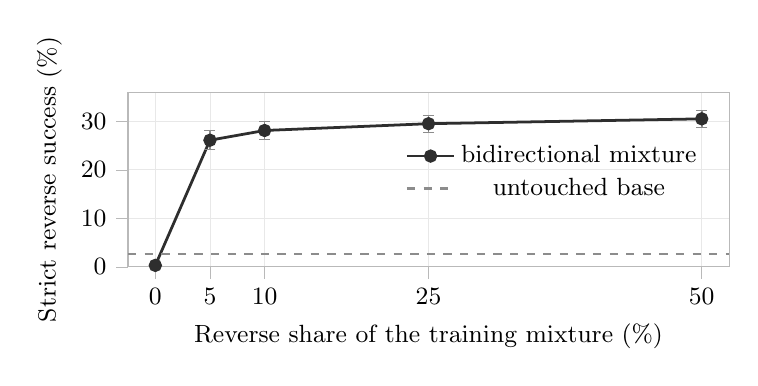
\begin{tikzpicture}
\begin{axis}[
  width=0.76\linewidth, height=3.8cm,
  xlabel={Reverse share of the training mixture (\%)},
  ylabel={Strict reverse success (\%)},
  xmin=-2.5, xmax=52.5, ymin=0, ymax=36,
  xtick={0,5,10,25,50}, ytick={0,10,20,30},
  tick align=outside, tick pos=left,
  axis line style={gray!55}, tick style={gray!55},
  grid=major, grid style={gray!18, line width=0.3pt},
  label style={font=\small}, tick label style={font=\small},
  legend style={font=\small, draw=none, fill=none, at={(0.97,0.32)},
                anchor=south east, cell picture=true},
]
\addplot[mark=*, mark size=1.9pt, line width=1pt, color=black!82,
         error bars/.cd, y dir=both, y explicit,
         error bar style={line width=0.6pt, color=black!45},
         error mark options={rotate=90, mark size=2pt, color=black!45}]
  coordinates {(0.0,0.3) +- (0,0.33) (5.0,26.1) +- (0,1.93) (10.0,28.1) +- (0,1.93) (25.0,29.5) +- (0,1.73) (50.0,30.5) +- (0,1.73)};
\addlegendentry{bidirectional mixture}
\addplot[dashed, line width=0.8pt, color=black!45, mark=none]
  coordinates {(-2.5,2.7) (52.5,2.7)};
\addlegendentry{untouched base}
\end{axis}
\end{tikzpicture}
\caption{\textbf{A little reverse data does almost all of the work.} Strict reverse
success against the reverse share of the training mixture, Qwen2.5-Coder-1.5B,
300 programs, 1\,500 graded trials per point. The zero-dose point is forward-only
SFT. Replacing just 5\% of the forward pairs with their own reverse recovers
26.1\% against 0.3\% for forward-only ---
85\%
of what a 50\% share recovers. The remaining climb is real but small
(+4.5 pp \ci{+3.2}{+5.8}
from 5\% to 50\%) and has flattened by 25\%
(+1.1 pp \ci{+0.0}{+2.1}
from 25\% to 50\%). Bars are 95\% cluster bootstraps by program; because the design is
paired, differences are quoted from the contrast table rather than read off the bars.}
\label{fig:dose}
\end{figure}

The curve rises steeply and then flattens. Replacing 5\% of the forward pairs recovers
$+25.7$ pp $[+23.9,+27.7]$ over forward-only training, which is 85\% of what a 50\% share
recovers; the remaining climb is $+4.5$ pp $[+3.2,+5.8]$ and has flattened by a quarter
share, where $50\%$ against $25\%$ is $+1.1$ pp $[+0.0,+2.1]$ with an interval touching zero.

\section{Limitations, in full}
\label{app:limits}

\textbf{Language and corpus.} The original study is Java over 10\,000 CodeNet programs,
while ours is Python over 7\,383 forward instances per epoch plus a JavaScript replication
of the four load-bearing arms at 1.5B. Two languages is evidence that the effect is not an
artifact of one, but neither is Java, so a Java-specific effect is not excluded.
\textbf{Scale and family.} Two sizes of one family, Qwen2.5-Coder 1.5B and 7B. The
original's strongest CFT numbers come from commercial models we cannot fine-tune the same
way, though our 7B result is at the tier of its open-source panel, and the 7B arms are
single-seed. 
\textbf{The general-capability probe overlaps the corpus}, as §\ref{sec:cost} sets out; a
held-out probe such as MBPP would settle it and we did not run one.


\textbf{Transform coverage.} String encryption, one of the original's three transforms and
its hardest, is quarantined in our corpus as a held-out family for a separate study and is
never trained on, so we report five conditions where the original reports three.

\textbf{Auxiliary pool ratio.} Our \arm{neg} pool is $0.76\times$ the size of the others
because negatives must survive execution verification. The token-share arithmetic in
Appendix~\ref{app:fidelity} bounds the auxiliary signal at $\approx$2.6\% of supervised
tokens even at parity, so the shortfall cannot plausibly account for a 30-point gap, but we
did not run the parity sweep.

\textbf{Pairing on HumanEval+.} The cost table is a single greedy pass per arm and only
aggregate counts were retained for the cells run before this draft, so §\ref{sec:cost}'s
grouping is a pattern across the arms rather than a set of per-pair significance tests.

\section{General-capability cost of the 1.5B dose ladder}
\label{app:dosecost}
\begin{center}\small
\begin{tabular}{lcc}
\toprule
arm & reverse share & HumanEval+ \texttt{plus} \\
\midrule
\arm{sft} & 0\% & .329 \\
\arm{mix5} & 5\% & .537 \\
\arm{mix10} & 10\% & .555 \\
\arm{mix25} & 25\% & .494 \\
\arm{mix50} & 50\% & .469 \\
\arm{rev} & 100\% & .585 \\
\arm{base} & n/a & .646 \\
\bottomrule
\end{tabular}
\end{center}
Qwen2.5-Coder-1.5B, 164 tasks, 0 scorer errors. The retained capability is \emph{not}
monotone in reverse share. \arm{mix5} and \arm{mix10} differ by 3 of 164 tasks, and
\arm{rev}, which has the largest reverse share, retains the most. We therefore draw no
dose-response conclusion on this axis at 1.5B. The 7B grouping in §\ref{sec:cost} does not
rest on these rows.

\section{Measured training budget (7B)}
\label{app:cost}
\begin{table}[h]
\centering\small
\caption{Measured per-epoch training budget, 7B Python corpus, relative to forward-only
SFT. Supervised tokens are the tokens the loss is actually computed on.}
\label{tab:cost}
\begin{tabular}{lrrrr}
\toprule
arm & instances & supervised tokens & sequence tokens ($\propto$ FLOPs) & steps \\
\midrule
\arm{fwd} \emph{(reference)} & 1.00$\times$ & 1.00$\times$ & 1.00$\times$ & 1.00$\times$ \\
\arm{fwd2x} & 1.00$\times$ & 1.00$\times$ & 1.00$\times$ & 2.00$\times$ \\
\textbf{\arm{mix50}} & \textbf{1.00$\times$} & \textbf{0.71$\times$} & \textbf{1.05$\times$} & \textbf{1.00$\times$} \\
\arm{rev} & 1.00$\times$ & 0.43$\times$ & 1.09$\times$ & 1.00$\times$ \\
\arm{flip} & 2.00$\times$ & 1.43$\times$ & 2.09$\times$ & 2.00$\times$ \\
\arm{cft} & 2.52$\times$ & \textbf{1.02$\times$} & \textbf{2.65$\times$} & 2.52$\times$ \\
\arm{cftflip} & 3.52$\times$ & 1.45$\times$ & 3.74$\times$ & 3.52$\times$ \\
\bottomrule
\end{tabular}
\end{table}

\section{Scoring quantities}
\label{app:metrics}
\begin{table}[h]
\centering\footnotesize
\caption{The quantities used to score a trial. \emph{Executes} is checked by running the
program on the test inputs that ship with it. $R$ returns 0 for a non-parsing output, since
the readability of a non-program is undefined and 0 is the only resolution that cannot
manufacture a success.}
\label{tab:metrics}
\begin{tabular}{llp{6.7cm}}
\toprule
symbol & range & meaning \\
\midrule
$\mathrm{parses}(\hat y)$ & $\{0,1\}$ & the output is non-empty and parses in the target
language \\
$S(a,b)$ & $[0,1]$ & CodeBLEU similarity between two programs
\citep{ren2020codebleu} \\
$R(a)$ & $[0,1]$ & readability, a weighted sum of identifier meaningfulness (0.55),
identifier length, line length and nesting depth (0.15 each) \\
$E(\hat y)$ & $\{0,1\}$ & the output executes and reproduces $x$'s outputs on every test input \\
\bottomrule
\end{tabular}
\end{table}

\section{The five obfuscating transforms}
\label{app:conditions}
\begin{table}[h]
\centering\small
\caption{The five obfuscating transforms. Each is applied on its own to the original
function. We keep the short codes because the appendix tables report results per
transform.}
\label{tab:conditions}
\begin{tabular}{llp{7.1cm}}
\toprule
code & family & what it does \\
\midrule
\arm{L1b} & identifier & renames identifiers to misleading names, so \texttt{count} might
become \texttt{buffer} \\
\arm{L1r} & identifier & renames identifiers to random strings such as \texttt{v\_a3f2} \\
\arm{L2} & identifier & renames identifiers to single letters and strips type annotations \\
\arm{S1} & structural & flattens control flow into a single dispatch loop driven by a state
variable \\
\arm{S2} & structural & inserts always-true tests and unreachable code \\
\bottomrule
\end{tabular}
\end{table}

\section{Strict reverse success by condition (7B)}
\label{app:bycond}
\begin{center}\small
\begin{tabular}{lccccc}
\toprule
arm & \arm{L1b} & \arm{L1r} & \arm{L2} & \textbf{\arm{S1}} & \textbf{\arm{S2}} \\
\midrule
\arm{base}  & .023 & .110 & .103 & .330 & .077 \\
\arm{sft}   & .000 & .000 & .000 & .000 & .000 \\
\arm{cft}   & .000 & .000 & .000 & .003 & .000 \\
\arm{fwd2x} & .000 & .000 & .000 & .003 & .000 \\
\arm{rev}   & .003 & .010 & .017 & \textbf{.817} & \textbf{.797} \\
\arm{flip}  & .017 & .013 & .023 & \textbf{.827} & \textbf{.797} \\
\arm{mix50} & .010 & .007 & .023 & \textbf{.803} & \textbf{.797} \\
\bottomrule
\end{tabular}
\end{center}
300 programs per cell, \texttt{simple} strategy, \texttt{e2\_budget\_qwen7b}. The
capability is almost entirely structural, since the identifier conditions are at or below
$2.3\%$ for every arm, including reverse-only training, because adversarial renaming
destroys information that no amount of reverse supervision can restore.

\section{Forward accuracy by condition (7B)}
\label{app:fwd}
\begin{center}\small
\begin{tabular}{lccccc}
\toprule
arm & \arm{L1b} & \arm{L1r} & \arm{L2} & \arm{S1} & \arm{S2} \\
\midrule
\arm{base}  & .950 & .960 & .963 & .933 & .837 \\
\arm{sft}   & .970 & .950 & 1.000 & .933 & 1.000 \\
\arm{cft}   & .973 & .960 & .997 & .947 & 1.000 \\
\arm{fwd2x} & .967 & .960 & 1.000 & .917 & 1.000 \\
\arm{rev}   & .940 & .950 & .957 & .970 & .820 \\
\arm{flip}  & .970 & .960 & 1.000 & .927 & .997 \\
\arm{mix50} & .973 & .957 & .990 & .883 & 1.000 \\
\bottomrule
\end{tabular}
\end{center}
Execution-verified forward success. \arm{flip} matches \arm{sft} everywhere;
bidirectionality is free in this direction too.

\section{Reverse prompting strategies (7B)}
\label{app:e7}
\begin{center}\small
\begin{tabular}{lccccr}
\toprule
system & \texttt{simple} & \texttt{few\_shot} & \texttt{cot} & \texttt{augmented} & range \\
\midrule
\arm{base} & 13.2 \ci{11.3}{15.3} & 18.1 \ci{15.7}{20.7} & \textbf{21.9} \ci{19.4}{24.5} & 21.4 \ci{18.8}{24.1} & 8.7 \\
\arm{sft} & 0.0 \ci{0.0}{0.0} & 1.6 \ci{1.0}{2.3} & \textbf{5.3} \ci{4.2}{6.3} & 5.1 \ci{4.1}{6.1} & 5.3 \\
\arm{cft} & 0.1 \ci{0.0}{0.2} & 0.5 \ci{0.1}{0.9} & \textbf{1.5} \ci{0.9}{2.1} & 1.2 \ci{0.7}{1.7} & 1.4 \\
\midrule
\arm{rev} & \textbf{32.9} \ci{31.5}{34.5} & 32.5 \ci{31.0}{34.0} & 32.5 \ci{31.0}{34.2} & 32.9 \ci{31.3}{34.4} & 0.4 \\
\arm{flip} & \textbf{33.7} \ci{32.1}{35.3} & 32.6 \ci{31.1}{34.1} & 32.8 \ci{31.2}{34.5} & 32.6 \ci{31.1}{34.1} & 1.1 \\
\arm{mix50} & \textbf{32.8} \ci{31.3}{34.4} & 31.3 \ci{29.6}{32.9} & 30.3 \ci{28.9}{31.9} & 31.7 \ci{30.0}{33.3} & 2.5 \\
\bottomrule
\end{tabular}
\end{center}
Strict reverse success (\%), cluster-bootstrap CIs by \texttt{program\_id}; all six arms
scored in one evaluation pass (\texttt{e7\_strategies\_qwen7b}), best strategy per arm in
bold. Both forward-only arms at their best strategy fall below the untuned base at its
worst. The bidirectional arms (lower block) are nearly flat across strategies while the
untuned base spans $8.7$ points, so capability installed by data does not depend on how it
is elicited.

\section{What the reverse criterion certifies (7B, \texttt{simple})}
\label{app:e8}
\begin{center}\small
\begin{tabular}{llrrrrrr}
\toprule
system & cond & paper \% & strict \% & id-rec (passes) & id-rec (all) & \textbf{lift} & floor \\
\midrule
\arm{base} & \arm{L1b} & 4.7 & 2.3 & 0.326 & 0.363 & $-0.037$ & 0.354 \\
\arm{base} & \arm{L1r} & 19.0 & 11.0 & 0.428 & 0.423 & $+0.005$ & 0.349 \\
\arm{base} & \arm{L2}  & 18.7 & 10.3 & 0.437 & 0.420 & $+0.017$ & 0.389 \\
\arm{base} & \arm{S1}  & 64.7 & 33.0 & 0.895 & 0.906 & $-0.011$ & 1.000 \\
\arm{base} & \arm{S2}  & 9.3 & 7.7 & 0.750 & 0.878 & $-0.127$ & 1.000 \\
\midrule
\arm{flip} & \arm{S1}  & 90.7 & 82.7 & 0.999 & 0.999 & $+0.001$ & 1.000 \\
\arm{flip} & \arm{S2}  & 79.7 & 79.7 & 1.000 & 0.999 & $+0.000$ & 1.000 \\
\arm{mix50} & \arm{S1} & 90.3 & 80.3 & 0.994 & 0.994 & $-0.000$ & 1.000 \\
\arm{mix50} & \arm{S2} & 79.7 & 79.7 & 0.999 & 0.999 & $-0.000$ & 1.000 \\
\bottomrule
\end{tabular}
\end{center}
\emph{floor} is the identifier recall of the obfuscated input itself, which is what echoing
scores.
\emph{lift} is id-recall among criterion-passing outputs minus id-recall among all outputs;
a lift near zero means the criterion certifies nothing about identifier recovery. The
structural conditions have a floor of exactly $1.000$, so identifier recall does not
discriminate there at all.

\section{Seed replication (1.5B, strict reverse success \%)}
\label{app:seeds}
\begin{center}\small
\begin{tabular}{lccc}
\toprule
arm & seed 17 & seed 42 & $\Delta$ \\
\midrule
\arm{sft}     & 0.4 & 0.4 & $+0.0$ \\
\arm{cft}     & 0.3 & 0.4 & $+0.1$ \\
\midrule
\arm{flip}    & 31.5 & 30.9 & $-0.6$ \\
\arm{rev}     & 31.5 & 31.2 & $-0.3$ \\
\arm{mix50}   & 30.6 & 30.0 & $-0.6$ \\
\arm{flipsym} & 30.5 & 30.8 & $+0.3$ \\
\midrule
\arm{base} \emph{(untuned anchor)} & 2.9 & 2.7 & $-0.2$ \\
\bottomrule
\end{tabular}
\end{center}
Identical harness, program set, criteria and decoding; the adapter seed is the only
difference. Columns come from two evaluation passes
(\texttt{e1\_qwen1.5b}, \texttt{e2\_seeds\_qwen1.5b}). The \arm{base} row has no seed and
is the same untouched model in both, so it calibrates the table. Roughly $0.2$ pp of the
movement in every other row is cross-pass noise rather than seed variance
(§\ref{sec:setup}).
The two arms carrying the paper's null move by $\leq0.1$. \arm{flipsym} trains \arm{flip}'s
mixture under a single shared system prompt and is a control against the two directions
being separable merely because they arrived under two personas.

\section{JavaScript replication (1.5B, strict reverse success \%)}
\label{app:js}
\begin{center}\small
\begin{tabular}{lcl}
\toprule
arm & JavaScript & contrast vs.\ Python \\
\midrule
\arm{base} & 3.8 \ci{2.5}{5.3} & (Python 2.9) \\
\arm{sft}  & 0.0 \ci{0.0}{0.0} & \arm{sft}$-$\arm{base} $-3.8$ \ci{-5.6}{-2.4} \\
\arm{cft}  & 0.4 \ci{0.0}{0.8} & \arm{cft}$-$\arm{sft} $+0.4$ \ci{+0.0}{+0.8} \\
\arm{mix50} & 30.3 \ci{27.4}{33.1} & \arm{mix50}$-$\arm{sft} $+30.3$ \ci{+28.3}{+32.5} \\
\arm{flip} & 30.4 \ci{27.5}{33.2} & \arm{flip}$-$\arm{mix50} $+0.1$ \ci{-0.2}{+0.5} \\
\bottomrule
\end{tabular}
\end{center}
167 programs, 835 graded trials per arm, same conditions and criteria as the Python
corpus. Every qualitative conclusion holds. Forward-only tuning lands below the untouched
model, the contrastive objective does not repair it, and the budget-matched bidirectional
arm captures the whole effect. Here it is statistically indistinguishable from the
doubled-data arm, whereas in Python the latter led by $+0.7$ pp.

% The NeurIPS paper checklist is a MAIN-CONFERENCE requirement. The ATTRIB call asks only
% for NeurIPS 2026 formatting, 3-6 body pages, and the appendix in the same PDF, and does
% not ask for the checklist. It is therefore not included; checklist.tex is left in the
% directory unused. If ATTRIB adds the requirement, re-add \input{checklist} here and fill
% its 16 \answerTODO entries.

\end{document}
